% ch22-cute-tiledmma.tex — CuTe（三）：TiledMMA 与 fragment（RFC-F F3，2026-09-11）
% \url 由 book.tex 的 hyperref 提供；单章独立编译时降级为可断行的 \ttfamily
\makeatletter
\providecommand{\urlchbrk}[1]{\@tfor\next:=#1\do{\next\allowbreak}}
\makeatother
\providecommand{\url}[1]{{\ttfamily\urlchbrk{#1}}}
\chapter{CuTe（三）：TiledMMA 与 fragment}\label{ch:22}

\section{本章导读}

第~\ref{ch:21}~章把「数据怎么搬」形式化成了 TiledCopy；本章处理另一半：
\textbf{计算怎么分给线程}。一条 \texttt{mma.\allowbreak{}sync.\allowbreak{}aligned.\allowbreak{}m16n8k16} 是硬件
给出的最小计算单元，它规定了 32 个 lane 各自的 4（或 8）个寄存器里装哪几个
元素；而一个真实 kernel 的 tile 远大于 $16\times8\times16$，于是「拿多个
MMA 原子去铺满 tile」这件事必须有个说法——这就是 \textbf{TiledMMA}：
原子 $\times$ 原子的排布 $\times$ 目标 tile 尺寸。

本章沿着第~\ref{ch:21}~章的 (thread, value) 语言继续：第~\ref{ch:21}~章里
TV 划分服务于\emph{搬运}，本章里 TV 划分服务于\emph{计算}，并且多出一个
维度——\textbf{fragment}（每个线程私有的寄存器数组）。核心问题是四个：
MMA 原子的 fragment 布局是什么（3.1 节）；TiledMMA 如何由「原子 $+$ warp
排布 $+$ tile 尺寸」构造出来（3.2 节）；partition 如何把 Tensor 切成
$(\mathrm{MMA}, \mathrm{MMA}_M, \mathrm{MMA}_K)$ 形状的片段
（3.3--3.5 节）；以及同一份寄存器为什么能在 QK 与 PV 两个不同的
TiledMMA 之间「原地复用」（4.3 节）。

\textbf{前置章节}：第~\ref{ch:20}~章（divide/zipped\_divide）、
第~\ref{ch:21}~章（Tensor 与 TV-layout）、第~\ref{ch:11}~章（m16n8k16 的
手写 fragment）、第~\ref{ch:15}~章（FA 的 P 复用背景）。\textbf{源码区间}：
ffpa\_attn.cuh~L31--64——\texttt{FFPAAttn\allowbreak{}Split\allowbreak{}DCu\allowbreak{}Te\allowbreak{}Traits} 的完整类型推导，
它是全书中唯一把\textbf{两个不同 tile 尺寸的 TiledMMA 写在同一个 traits 里}
的样本（QK 用 $64\times64\times16$ 一次覆盖 $S$，PV 用 $64\times16\times16$
控制累加器）。使用点引 ffpa\_attn.cuh~L151--158、L257--264、L300--305、
L339--345（cp.async 版本的 fragment 流转，与 TMA+WS 版逐行一致）。
\textbf{编译宏}：\texttt{NOTES\_\allowbreak{}V2\_\allowbreak{}ENABLE\_\allowbreak{}CUTE}。配套最小测试
\texttt{book/\allowbreak{}tests/\allowbreak{}ch22\_\allowbreak{}tiled\_\allowbreak{}mma.cu}：host 端 partition 一致性断言。

\section{问题与动机}

先从一条 mma 指令说起。\texttt{mma.\allowbreak{}sync.\allowbreak{}aligned.\allowbreak{}m16n8k16} 不是一个线程的
算术指令，而是\textbf{一个 warp 的集体动作}：32 个 lane 各自从自己的寄存器里
拿出 A、B 的一小片，硬件把它们拼成 $16\times16$ 与 $8\times16$ 的矩阵送进
tensor core，算完再把 $16\times8$ 的 C 分散写回 32 个 lane 的寄存器。所以
写 mma 的第一件事是回答「\textbf{我这条 lane 的寄存器里该装哪几个元素}」——
以 C（$16\times8$）为例，thread 0 负责 $(0,0)$、$(0,1)$、$(8,0)$、$(8,1)$
四个位置，thread 4 负责 $(1,0)$、$(1,1)$、$(9,0)$、$(9,1)$，以此类推
（@竹熙佳处《写给大家看的 CuTe 教程：tiled mma》把这张 thread-data 映射图
作为理解的起点）。

这些坐标不是自由选择的，而是 PTX 规定的 fragment 布局。回忆第~\ref{ch:11}~章
手写 HGEMM 的寄存器清单：一条 m16n8k16 要 4 个 A 寄存器（8 个 half）、
2 个 B 寄存器（4 个 half）、4 个 C 寄存器（float）。以 A（$16\times16$，
列主序的 $(m,k)$）为例，lane 与元素的对应是

\begin{equation}
  \mathrm{row} = \Bigl\lfloor\frac{\mathrm{lane}}{4}\Bigr\rfloor,\qquad
  \mathrm{col} = 2\,(\mathrm{lane}\bmod 4) + (0\ \text{或}\ 1),
  \label{eq:22-ptx-a}
\end{equation}

外加「$+8$ 行」与「$+8$ 列」两套偏移把 8 个 half 填满。B（$8\times16$）也是
类似的故事。手写版（第~\ref{ch:11}~章）的做法是：把这些式子连同 ldmatrix
的 lane 地址表一起写在 kernel 里。这条路能走通，但三个痛点随规模一起放大：

\begin{itemize}
  \item \textbf{换一条指令就要重查一次手册}。m16n8k8（fp16 半 K）、
        m16n8k32（int8）的 fragment 排布各不相同；每换一次，寄存器分配与
        地址算术都要重算，改对与否只能靠再跑一遍正确性测试；
  \item \textbf{跨架构可能要重写}。Volta 的 fragment 排布与 Ampere 不同，
        硬件换代意味着手推的公式作废——这是「CUDA $+$ PTX」路线的固有风险；
  \item \textbf{放大到 tile 级别没有脚手架}。真实 kernel 的 tile 远大于
        $16\times8\times16$：要么多起几个 warp 沿 M/N/K 排开（\emph{并行}
        维度），要么让一个 warp 循环执行多条 mma（\emph{串行}维度）。这两层
        「重复」的坐标运算——谁负责哪块、重复多少次、寄存器怎么编号——
        手推起来极易出错。
\end{itemize}

CuTe 对这三条痛点的回应可以概括成一句：\textbf{把 atom 的 thread-data 映射
本身变成一个 layout，然后让「重复」成为 layout 的乘法}。动机就位后，本章
沿着这条线索往下走。

把上述规则放到 FFPA 上实例化。FFPA 的 QK 步骤要算
$S_{64\times64} = Q_{64\times64} K^T_{64\times64}$（每个 d-chunk），PV 步骤
要算 $O_{64\times64} = P_{64\times64} V_{64\times64}$——两个 $64\times64$ 的
结果，每个线程要用多条 m16n8k16 拼出来。「拼」的规则至少包括：

\begin{itemize}
  \item \textbf{warp 怎么分}：QK 用 4 个 warp 沿 M 方向切（每个 warp 16 行），
        还是 $2\times2$ 网格？不同选择决定 A/B fragment 的重复因子
        （第~\ref{ch:21}~章式~(21-dup)）；
  \item \textbf{每个 warp 内部怎么重复}：一个 warp 覆盖 16 行 $\times$ 64 列时，
        N 方向要 8 个原子；这 8 个原子的寄存器块怎么编号；
  \item \textbf{K 方向怎么切}：tile 的 K 长度是 64，而原子是 16，于是 fragment
        多出一个 $\mathrm{MMA}_K$ mode；
  \item \textbf{两个不同形状的 tile 怎么并存}：QK 要大 tile（省循环、提高
        计算密度），PV 要小 N tile（控制 acc\_O 寄存器）——它们必须共享
        同一套线程/值编号。
\end{itemize}

CuTe 的答案是把这四件事压进一个类型：\texttt{Tiled\allowbreak{}MMA\allowbreak{}<MMA\_\allowbreak{}Atom,\allowbreak{}
Atom\allowbreak{}Layout\allowbreak{}MNK,\allowbreak{} Permutation\allowbreak{}MNK>}。一个 TiledMMA 实例只回答两个问题：
\textbf{「这个 tile 有哪些 (线程, 值) 位置」}与\textbf{「给定一个 Tensor，
每个线程的 fragment 是什么形状」}——@竹熙佳处把动机总结成「给定任意一条
mma 指令，都能方便地推导出每个线程该从 data tile 里取哪一部分」，与这里的
两个问题是同一件事的两种说法。本章要验证的，就是这两个回答在 FFPA 的
具体配置下能否用手推公式复现——不能复现就说明没读懂。

\section{数学原理}

\subsection{MMA 原子：一条指令的 thread-data 映射}

先回到最小尺度：一条指令、一个 warp。C 的 thread 0 拿 $(0,0)$、$(0,1)$、
$(8,0)$、$(8,1)$，thread 4 拿 $(1,0)$、$(1,1)$、$(9,0)$、$(9,1)$——这张
thread-data 对照表就是原子的全部内容。CuTe 用一个 traits 类把它写成类型
（\texttt{MMA\_\allowbreak{}Traits\allowbreak{}<Op>}），FFPA 用到的
\texttt{SM80\_\allowbreak{}16x8x16\_\allowbreak{}F32\allowbreak{}F16\allowbreak{}F16\allowbreak{}F32\_\allowbreak{}TN} 实测（CUTLASS v4.6.1）为：

\begin{center}
\footnotesize
\begin{tabular}{@{}lll@{}}
  \toprule
  成员 & 值 & 含义 \\
  \midrule
  \texttt{Shape\_MNK} & $(16,8,16)$ & 原子覆盖的 $M\times N\times K$ \\
  \texttt{ThrID} & $\mathrm{Layout}\_32$ & 原子用 32 个线程（一个 warp） \\
  \texttt{LayoutA\_TV} & $((4,8),(2,2,2)){:}((32,1),(16,8,128))$ & $(\mathrm{thr},\mathrm{val})\to$ A 的扁平坐标 \\
  \texttt{LayoutB\_TV} & $((4,8),(2,2)){:}((16,1),(8,64))$ & $(\mathrm{thr},\mathrm{val})\to$ B 的扁平坐标 \\
  \texttt{LayoutC\_TV} & $((4,8),(2,2)){:}((32,1),(16,8))$ & $(\mathrm{thr},\mathrm{val})\to$ C 的扁平坐标 \\
  \bottomrule
\end{tabular}
\end{center}

这些 layout 的 codomain 是\textbf{扁平坐标}：A 的扁平量是 $m + 16k$（M 最快），
B 是 $n + 8k$，C 是 $m + 16n$——三者都按「第一个 mode 最快」的 colex 约定
（第~\ref{ch:20}~章式~(20-colex-decomp)）线性化。换句话说，三份
\texttt{Layout*\_TV} 就是「thread-data 映射」的类型化写法：
\textbf{给它一个 (lane, 值编号)，它返回该元素在原子小矩阵里的扁平坐标}。
以 \texttt{LayoutC\_TV} $=((4,8),(2,2)){:}((32,1),(16,8))$ 为例，用映射
语言说：lane 被拆成 $(\mathrm{lane}\bmod4,\ \lfloor\mathrm{lane}/4\rfloor)$
两维，低位那维的 stride 是 $32$——因为 C 的扁平坐标按 $m+16n$ 线性化，
$32$ 恰好是\emph{两列}（列号加 2），高位那维 stride 是 $1$（行号加 1）；
值编号的两维 stride 为 $16$（列加 1）与 $8$（行加 8，正是装填用的「$+8$ 行」
偏移）。把 stride 反解回坐标，就得到三条可以独立验证的公式
（lane $=\mathrm{thr}$，值编号 $v$ 按 colex 拆位）：

\begin{align}
  \textbf{A}:\quad &m = \Bigl\lfloor\frac{\mathrm{lane}}{4}\Bigr\rfloor + 8\,d_1,
  \quad k = 2\,(\mathrm{lane}\bmod 4) + d_0 + 8\,d_2, \label{eq:22-atom-a}\\
  \textbf{B}:\quad &n = \Bigl\lfloor\frac{\mathrm{lane}}{4}\Bigr\rfloor,
  \quad k = 2\,(\mathrm{lane}\bmod 4) + d_0 + 8\,d_1, \label{eq:22-atom-b}\\
  \textbf{C}:\quad &m = \Bigl\lfloor\frac{\mathrm{lane}}{4}\Bigr\rfloor + 8\,d_1,
  \quad n = 2\,(\mathrm{lane}\bmod 4) + d_0, \label{eq:22-atom-c}
\end{align}

其中 $(d_0,d_1,d_2)$ 是值编号 $v$ 在原子值 mode 上的 colex 分解
（A：$v=d_0+2d_1+4d_2$，8 个 half；B/C：$v=d_0+2d_1$，4 个元素）。
式~\eqref{eq:22-atom-a}--\eqref{eq:22-atom-c} 与 PTX 文档给的 m16n8k16
fragment 图完全一致。例如 lane 0 的 A 是
\begin{equation*}
  \{(0,0),(0,1),(8,0),(8,1),(0,8),(0,9),(8,8),(8,9)\},
\end{equation*}
lane 31 是 $\{(7,6),(7,7),(15,6),(15,7),(7,14),\dots\}$——\textbf{CuTe 没有
另立一套约定，它就是 PTX 约定的类型化表达}。本章测试 case~A 对三条公式在
32 个 lane 上逐点核对，并用「32 线程 $\times$ 每线程值数 $=$ 原子元素数」
验证守恒（A：$32\times8=256=16\times16$；B：$32\times4=128=8\times16$；
C：$32\times4=128=16\times8$）。

\textbf{单 warp 演练：\texttt{partition\_\allowbreak{}fragment\_\allowbreak{}A/\allowbreak{}B/\allowbreak{}C} 给出什么？}
把原子包成最小的 TiledMMA（warp 排布 $(1,1,1)$，tile 参数就是原子形状），
对一个 $16\times16$ 的 A、$8\times16$ 的 B、$16\times8$ 的 C 调用三个
partition：tile 不放大、线程不增，每线程拿到的就是原子自身的一份 fragment——
A 为 $(8,1,1)$（8 个 half）、B 为 $(4,1,1)$、C 为 $(4,1,1)$，与
第~\ref{ch:11}~章手写版的寄存器清单逐一对应。这不是巧合：\textbf{partition
在「单 warp $+$ 单原子」的退化情形下输出的就是 PTX fragment 本身}；它真正的
价值——tile 放大后的 remainder 与多 warp 的重复因子——要到 3.2--3.3 节才
显现。

\subsection{TiledMMA：原子、排布、tile 三件套}

再回到动机里那两层「重复」：\textbf{并行维度}（多起执行器）与\textbf{串行
维度}（一个执行器循环执行）。CuTe 把两者装进
\texttt{make\_\allowbreak{}tiled\_\allowbreak{}mma\allowbreak{}(atom,\allowbreak{} Atom\allowbreak{}Layout\allowbreak{}MNK,\allowbreak{} Permutation\allowbreak{}MNK)} 的三个参数：
原子是硬件粒度，第二个参数是\textbf{warp 排布}（哪个 warp 覆盖哪个原子位置，
负责并行重复），第三个是\textbf{目标 tile 尺寸}（含 K，决定一个 threadblock
一次「打出去」的计算块）。内核把两者合成为

\begin{equation}
  \mathrm{ThrLayoutVMNK} = \mathrm{tiled\_product}(\mathrm{ThrID},\
  \mathrm{AtomLayoutMNK}) \ \cong\ (\mathrm{ThrV},\mathrm{ThrM},
  \mathrm{ThrN},\mathrm{ThrK}) ,
  \label{eq:22-thr-vmnk}
\end{equation}

实测（FFPA 的 QK）：
$\mathrm{thr\_layout\_vmnk} = (32,4,1,1){:}(1,32,0,0)$——$\mathrm{ThrV}=32$
是 warp 内部线程（stride 1），$\mathrm{ThrM}=4$ 是 4 个 warp 沿 M 排列
（stride 32）。同时 tile 的尺寸由

\begin{equation}
  \mathrm{tile\_size}_I = \mathrm{size}\bigl(\mathrm{permutation\_mnk}\langle I\rangle\bigr),
  \qquad
  \mathrm{permutation\_mnk}\langle I\rangle =
  \begin{cases}
    \text{显式给定}, & \text{非下划线},\\[2pt]
    \mathrm{atom}_I \times \mathrm{Thr}_I, & \text{否则},
  \end{cases}
  \label{eq:22-tile-size}
\end{equation}

给出：QK 实测 $\mathrm{tile\_size} = (64,64,16)$，PV 为 $(64,16,16)$
（FFPA 两者都显式给定）。式~\eqref{eq:22-tile-size} 的第二行是「不显式
给时会怎么算」：$\mathrm{tile}_I = \mathrm{atom}_I \times \mathrm{Thr}_I$，
原子长度乘该方向的 warp 组数（M 对应
$\mathrm{ThrM}$、N 对应 $\mathrm{ThrN}$、K 对应 $\mathrm{ThrK}$）。

用映射语言说：\texttt{Thr\allowbreak{}Layout\allowbreak{}VMNK} 把\textbf{线程编号}拆成
$(\mathrm{ThrV},(\mathrm{ThrM},\mathrm{ThrN},\mathrm{ThrK}))$ 四层——先看
warp 内部（$\mathrm{ThrV}$），再看「第几个 warp 落在哪个方向」。
\textbf{「谁并行、谁重复」这两个问题的答案，就藏在把线程编号拆成 VMNK 的
那一刻。}

一个自然的疑问是：既然 warp 排布 $+$ 原子尺寸已经能划分 tile，为什么还要
第三个（tile）参数？@竹熙佳处给出两条理由，读 tiled mma 时值得记住。其一
是\textbf{拷贝粒度}：后续 S2R/R2S tiled copy 把这个参数描述的块整体当作拷贝
单位，N 方向留大一倍（每个 warp 16 而非 8）才能用上 \texttt{ldsm.x4} 一类的
宽指令；其二是\textbf{重排的余地}：tile 参数本质是一个 layout，高级用法可以
借助它的 stride 把多条指令算出的数据在寄存器里重新排列——这正是
\texttt{Permutation\allowbreak{}MNK} 这个名字的由来。常规场景把它当 tile 尺寸读即可。

\subsection{q 的推导链：从 tile 到 fragment}

真正的工作在 \texttt{thrfrg\_\allowbreak{}A/\allowbreak{}B/\allowbreak{}C} 里，它是四步 layout 代数
（第~\ref{ch:20}~章的全部工具在这里合体）。四步走的是一条固定流水线：
\textbf{先按 tile 切、再按原子切、把原子坐标换成 (线程, 值)、最后按 warp
排布把线程剥出来}。以 A 为例（B/C 只是把 mode 换成 $(N,K)$ / $(M,N)$）：

\begin{align}
  &\text{(1) 按 tile 分块} &
  T_1 &= \mathrm{logical\_divide}\bigl(A,\!(\mathrm{perm}_M, \mathrm{perm}_K)\bigr),
  \label{eq:22-thrfrg-1}\\
  &\text{(2) 按原子切分} &
  T_2 &= \mathrm{zipped\_divide}\bigl(T_1,\ (\mathrm{atom}_M,
  \mathrm{atom}_K)\bigr) = \bigl((A_M,A_K),(R_M,R_K)\bigr),
  \label{eq:22-thrfrg-2}\\
  &\text{(3) 原子坐标}\!\to\!(\text{线程},\text{值}) &
  T_3 &= T_2 \circ \mathrm{LayoutA\_TV} = \bigl((\mathrm{ThrV},
  \mathrm{FrgV}),(R_M,R_K)\bigr),
  \label{eq:22-thrfrg-3}\\
  &\text{(4) 按 warp 排布切分} &
  T_4 &= \mathrm{zipped\_divide}\bigl(T_3, (\_,
  (\mathrm{ThrM},\mathrm{ThrK}))\bigr) \notag\\
  & & &= \bigl((\mathrm{ThrV},
  (\mathrm{ThrM},\mathrm{ThrK})),(\mathrm{FrgV}, (R'_M, R'_K))\bigr).
  \label{eq:22-thrfrg-4}
\end{align}

用一句话概括这条链：\textbf{把 tensor 按坐标层层切开，切到只剩原子的 MN
坐标，再经 \texttt{LayoutA\_TV} 换成 (线程, 值)}。四步里的三个量各司其职：
第 (1) 步的 $\mathrm{perm}$ 决定「一个 tile 多大」，第 (2) 步的
$\mathrm{atom}$ 决定「一条指令多大」，第 (4) 步的
$\mathrm{ThrM/ThrK}$ 决定「多少 warp 分摊」——正是 3.2 节三件套的第三次
出场；对线程 $t$ 来说，前三步的结果人人相同，只有第 (4) 步把他自己摘出来。

把第 (4) 步的线程坐标 $(\mathrm{ThrV},\mathrm{ThrM},\mathrm{ThrK})$ 用
\texttt{get\_\allowbreak{}slice\allowbreak{}(t)} 固定住，剩下的就是该线程的 fragment 形状：

\begin{equation}
  \mathrm{fragment} = \bigl(\underbrace{\mathrm{FrgV}}_{\mathrm{MMA}},\
  \underbrace{R'_M}_{\mathrm{MMA}_M},\ \underbrace{R'_K}_{\mathrm{MMA}_K}\bigr) ,
  \label{eq:22-fragment}
\end{equation}

$R'_M = R_M/\mathrm{ThrM}$、$R'_K = R_K/\mathrm{ThrK}$ 是「warp 分完之后每个
线程还要重复多少个原子」。以 FFPA 的 QK（tile $64\times64\times16$、
$\mathrm{AtomLayout}=(4,1,1)$）在 $64\times64$ 的 Q 上为例逐项算：

\begin{itemize}
  \item (1)  $\mathrm{perm} = (64,16)$：$T_1 = ((64,16),(1,4))$；
  \item (2)  $\mathrm{atom}=(16,16)$：$T_2 = ((16,16),(4,4))$，即
        $R_M = 64/16 = 4$、$R_K = 64/16 = 4$；
  \item (3)  $\mathrm{LayoutA\_TV}$ 把 $(16,16)$ 变成 $(\mathrm{ThrV}=32,
        \mathrm{FrgV}=8)$：$T_3 = ((32,8),(4,4))$；
  \item (4)  $\mathrm{ThrM}=4$：$(\mathrm{FrgV},(R'_M,R'_K)) = (8,(1,4))$。
\end{itemize}

于是 $\mathrm{MMA}=8$、$\mathrm{MMA}_M = 1$、$\mathrm{MMA}_K = 4$，
fragment 大小 $8\times1\times4 = 32$——与本章测试 case~C 的实测
\texttt{\allowbreak{}(\allowbreak{}(2,\allowbreak{}2,\allowbreak{}2),\allowbreak{}1,\allowbreak{}4)} 完全一致（$(2,2,2)$ 是 8 的嵌套写法）。
测试同时对 B 与 C 复算了这条链：QK 的 B 在 $(64,64)$ 上得
$(4,8,4)$（$=128$ 个 half/线程，因为 4 个 M-warp 各持一份完整 B，重复因子 4，
式~\eqref{eq:22-dup}）；C 得 $(4,1,8) = 32$（无重复，$4096/128$）。四步
推导链的 shape 演化见图~\ref{fig:22-thrfrg-chain}。

\begin{figure}[H]
\centering
\begin{tikzpicture}[font=\tiny]
  \begin{scope}
    \foreach \fk in {0,...,3}{
      \ifnum\fk=0 \def\cfill{gray!45} \else \def\cfill{gray!10} \fi
      \fill[\cfill] ({0.6*\fk},0) rectangle ({0.6*\fk+0.6},{-2.4});
    }
    \draw[thin] (0,0) grid[xstep=0.6cm, ystep=0.3cm] (2.4,-2.4);
    \draw[very thick] (0,0) rectangle (2.4,-2.4);
    \node[font=\tiny, rotate=90] at (0.3,-1.2) {tile $(64,16)$};
    \node[font=\tiny, rotate=90] at (1.5,-1.2) {rest $(1,4)$：4 个 K 切片};
    \node[anchor=south, font=\tiny] at (1.2,0.42) {$A$：$64\times64$，perm $=(64,16)$};
    \node[anchor=south, font=\tiny\bfseries] at (1.2,0.14) {(1) logical\_divide};
    \node[anchor=north, font=\tiny] at (1.2,-2.55) {$T_1=((64,16),(1,4))$};
  \end{scope}
  \draw[->, very thick] (2.6,-1.2) -- (3.3,-1.2);
  \begin{scope}[shift={(3.5,0)}]
    \foreach \am in {0,...,3}{
      \foreach \ak in {0,...,3}{
        \pgfmathtruncatemacro{\pk}{mod(\am+\ak,2)}
        \ifnum\pk=0 \def\cfill{gray!22} \else \def\cfill{gray!52} \fi
        \fill[\cfill] ({0.33*\ak},{-0.6*\am}) rectangle ({0.33*\ak+0.33},{-0.6*\am-0.6});
      }
    }
    \draw[thin] (0,0) grid[xstep=0.33cm, ystep=0.6cm] (1.32,-2.4);
    \draw[very thick] (0,0) rectangle (1.32,-2.4);
    \node[anchor=south, font=\tiny] at (0.66,0.42) {atom $(16,16)$};
    \node[anchor=south, font=\tiny\bfseries] at (0.66,0.14) {(2) zipped\_divide};
    \node[anchor=north, font=\tiny, align=center] at (0.66,-2.55)
      {$T_2=((16,16),(4,4))$，$R_M{=}R_K{=}4$\\（棋盘 $=$ atom 身份）};
  \end{scope}
  \draw[->, very thick] (5.0,-1.2) -- (5.4,-1.2);
  \begin{scope}[shift={(5.6,0)}]
    \foreach \gm/\gk in {0/0,0/1,0/8,0/9,8/0,8/1,8/8,8/9}{
      \fill[gray!65] ({0.135*\gk},{-0.135*\gm}) rectangle ({0.135*\gk+0.135},{-0.135*\gm-0.135});
    }
    \draw[thin] (0,0) grid[xstep=0.135cm, ystep=0.135cm] (2.16,-2.16);
    \draw[very thick] (0,0) rectangle (2.16,-2.16);
    \node[anchor=south, font=\tiny] at (1.08,0.42) {atom $(16,16)\to(\mathrm{thr},\mathrm{val})$};
    \node[anchor=south, font=\tiny\bfseries] at (1.08,0.14) {(3) $\circ$ LayoutA\_TV};
    \node[anchor=north, font=\tiny, align=center] at (1.08,-2.3)
      {深色 8 格 $=$ lane 0 的 FrgV：$\{(0,0),(0,1),(8,0),(8,1),$\\
       $(0,8),(0,9),(8,8),(8,9)\}$（式~\eqref{eq:22-atom-a}）};
    \node[anchor=north, font=\tiny] at (1.08,-3.1) {$T_3=((32,8),(4,4))$};
  \end{scope}
  \draw[->, very thick] (7.95,-1.2) -- (8.4,-1.2);
  \begin{scope}[shift={(8.6,0)}]
    \foreach \am in {0,...,3}{
      \foreach \ak in {0,...,3}{
        \ifnum\am=1 \def\cfill{gray!68} \else \def\cfill{gray!25} \fi
        \fill[\cfill] ({0.33*\ak},{-0.6*\am}) rectangle ({0.33*\ak+0.33},{-0.6*\am-0.6});
      }
    }
    \draw[thin] (0,0) grid[xstep=0.33cm, ystep=0.6cm] (1.32,-2.4);
    \draw[very thick] (0,0) rectangle (1.32,-2.4);
    \draw[thick] (0,-0.6) -- (1.32,-0.6);
    \draw[thick] (0,-1.2) -- (1.32,-1.2);
    \draw[thick] (0,-1.8) -- (1.32,-1.8);
    \draw[->, thick] (1.5,-0.9) -- (1.36,-0.9);
    \node[anchor=west, font=\tiny, align=left] at (1.56,-0.9)
      {warp $w$（thrM $=w$）的行带；\\get\_slice$(t)$ 后 $R'_M{=}1$、$R'_K{=}4$};
    \node[anchor=south, font=\tiny] at (0.66,0.42) {$(\_,(\mathrm{ThrM},\mathrm{ThrK}))=(4,1)$};
    \node[anchor=south, font=\tiny\bfseries] at (0.66,0.14) {(4) zipped\_divide};
    \foreach \ak in {0,...,3}{
      \draw[fill=gray!55, thick] ({0.33*\ak},-3.35) rectangle ({0.33*\ak+0.33},-3.05);
      \node[font=\tiny] at ({0.33*\ak+0.165},-3.2) {8};
    }
    \node[anchor=east, font=\tiny] at (-0.1,-3.2) {FrgV};
    \node[anchor=north, font=\tiny, align=center] at (0.66,-3.5)
      {$(\mathrm{FrgV},(R'_M,R'_K))=(8,(1,4))$\\$\mathrm{MMA}_K{=}4$ 个 atom $\times$ 每原子 8 half};
  \end{scope}
  \node[anchor=north west, font=\tiny, align=left] at (0,-4.35)
    {fragment $=(\mathrm{MMA},\mathrm{MMA}_M,\mathrm{MMA}_K)=(8,1,4)$：每线程
     $8\times1\times4=32$ half；\\ $\times\,128$ 线程 $=4096=64\times64$
     （双射，case~C/D）；\\ B/C 同链只换 mode：B 得 $(4,8,4)$（4 倍重复）、
     C 得 $(4,1,8)$。};
\end{tikzpicture}
\caption{thrfrg\_A 四步推导链（式~\eqref{eq:22-thrfrg-1}--\eqref{eq:22-thrfrg-4}）
在 FFPA QK（tile $64\times64\times16$、AtomLayout $(4,1,1)$、Q 为
$64\times64$）上的 shape 演化：(1) logical\_divide 按 tile 切出 $(64,16)$
与 4 个 K 切片；(2) zipped\_divide 按 atom $(16,16)$ 切成 $4\times4$ 个
原子块；(3) 复合 LayoutA\_TV 把原子内坐标换成（线程, 值），深色 8 格即
lane 0 的 FrgV；(4) 按 $(\mathrm{ThrM},\mathrm{ThrK})=(4,1)$ 剥出 warp 行带，
get\_slice$(t)$ 后每线程 fragment $=(8,(1,4))=32$ half（右下：FrgV $=8$
$\times$ $\mathrm{MMA}_K=4$）。}
\label{fig:22-thrfrg-chain}
\end{figure}

\begin{equation}
  \text{A 的重复因子} = \#\{\text{N-warp}\},\qquad
  \text{B 的重复因子} = \#\{\text{M-warp}\},\qquad
  \text{C 无重复} .
  \label{eq:22-dup}
\end{equation}

\subsection{守恒与 tile 循环}

把三个 fragment 的每线程元素数乘以线程数，得到的是「数据被读了几遍」：
C 恰好等于 tile 元素数（$128\times32 = 4096 = 64\times64$，双射），
A 也是（$\mathrm{ThrK}=1$ 时无 K-warp 重复），B 是 4 倍。这条账在选 tile 时
必须算清楚：B 的 4 倍重复意味着 128 个 half/线程的寄存器开销——它不占
smem，但吃寄存器预算。守恒式也是最便宜的自检：两边对不上，说明有数据没有
线程负责、或有线程在空转（本章测试 case D 就是这条账的逐点版本）。

当 tensor 比 tile 大时，partition 会多出「tile 重复」mode：$64\times64$ 的
tile 作用在 $64\times256$ 的 C 上，$\mathrm{MMA}_N$ 从 8 变成 32。这不是新
机制，只是式~\eqref{eq:22-thrfrg-1} 的 $T_1$ 多留了一层 remainder。
\texttt{gemm\allowbreak{}(tiled\_\allowbreak{}mma,\allowbreak{} A,\allowbreak{} B,\allowbreak{} C)} 会在这一层 remainder 上循环——这正是
第~\ref{ch:21}~章 kernel 里「只显式展开 K 循环、M/N 交给 \texttt{cute::gemm}」
的原因（hgemm.cuh~L925--937 的注释）。

\subsection{get\_slice：线程坐标的三层解构}

一行调用 \texttt{thr\_\allowbreak{}mma =\allowbreak{} tiled\_\allowbreak{}mma.\allowbreak{}get\_\allowbreak{}slice\allowbreak{}(t)} 就能完成线程坐标的
三层解构：把整数 $t$ 按式~\eqref{eq:22-thr-vmnk} 的 layout 分解成
$(\mathrm{ThrV},(\mathrm{ThrM},\mathrm{ThrK}))$（C 用 $(\mathrm{ThrV},(\mathrm{ThrM},\mathrm{ThrN}))$）。
FFPA 的 QK：$\mathrm{ThrLayoutVMNK} = (32,4,1,1){:}(1,32,0,0)$，于是

\begin{equation}
  \mathrm{ThrV} = t \bmod 32,\qquad \mathrm{ThrM} = \Bigl\lfloor\frac{t}{32}
  \Bigr\rfloor \bmod 4 , \qquad \mathrm{ThrK} = 0 .
  \label{eq:22-get-slice}
\end{equation}

本测试 case~E 用它验证了「warp 边界」：warp $w$ 的 C fragment 恰好覆盖
$M$ 方向的第 $16w$ 到 $16w+15$ 行，四个 warp 的行带互不重叠且并集为
$[0,64)$——这就是 $\mathrm{ThrM}=4$、$\mathrm{atom}_M=16$ 的直接推论。
\texttt{get\_\allowbreak{}thread\_\allowbreak{}slice} 是 \texttt{get\_slice} 的别名（v4.6.1 实测同一
实现），旧教程里两个名字都可能出现。

\section{设计与实现}

\subsection{FFPA traits：两个 TiledMMA 的完整推导}

先看源码区间本体——它短小但信息密度极高，每一行都对应 3.3 节的一个量：

\lstinputlisting[linerange={31-62},firstnumber=auto,breakatwhitespace=true,
  title={ffpa\_attn.cuh L31-62（FFPAAttnSplitDCuTeTraits：QK 与 PV 双 TiledMMA）}]{../ffpa_attn.cuh}

逐项解读：

\begin{itemize}
  \item \texttt{Smem\allowbreak{}Layout\allowbreak{}Atom =\allowbreak{} GMMA::\allowbreak{}Layout\_\allowbreak{}K\_\allowbreak{}SW128\_\allowbreak{}Atom\allowbreak{}<half>}：smem 的
        布局原子（第~\ref{ch:23}~章的 SW128），本 traits 只用它定义
        Q/KV 的 smem 视图；$64\times64$ 的 tile 实测
        \texttt{cosize} $=4096$（与 $64\times64$ 个 half 一致，无空洞）；
  \item \texttt{Smem\allowbreak{}Layout\allowbreak{}Vt}：把 KV 的布局\emph{转置}成「$d$ 为行、$kv$ 为列」，
        供 PV 的 B（$V^T$）使用——这是 ch19 讲过的「$V$ 以转置形态喂给
        MMA」的布局表达；
  \item \texttt{Mma\allowbreak{}Atom =\allowbreak{} MMA\_\allowbreak{}Atom\allowbreak{}<SM80\_\allowbreak{}16x8x16\_\allowbreak{}F32\allowbreak{}F16\allowbreak{}F16\allowbreak{}F32\_\allowbreak{}TN>}：
        F32 累加（attention 的数值要求），与 3.1 节的 fragment 一致；
  \item \texttt{TiledMmaQK}：$\mathrm{AtomLayoutMNK} = (4,1,1)$（4 个 warp
        沿 M 切）、$\mathrm{PermutationMNK} = (64,64,16)$。实测
        $\mathrm{tile\_size} = (64,64,16)$、线程数 $128$；
  \item \texttt{TiledMmaPV}：同样的 warp 排布，tile 换成 $(64,16,16)$——
        N 方向只留 16，因为 acc\_O 要常驻寄存器；
  \item 两个 \texttt{Copy\_Atom}：\texttt{LDSM\_N}（正常读）与
        \texttt{LDSM\_T}（转置读 V），它们是第~\ref{ch:21}~章
        \texttt{make\_\allowbreak{}tiled\_\allowbreak{}copy\_\allowbreak{}B} 的原子参数。
\end{itemize}

\textbf{为什么 QK 用 $64\times64$ 的 tile？}因为 $S$ 的 N 方向（KV 方向）正好
是 64——一次 TiledMMA 覆盖整个 $S$，省掉 N-tile 循环。实测
$\mathrm{MMA}_N = 8$（$8$ 个 $8$ 列的原子），全部落在同一个 warp 内、
同一批寄存器里；这对应注释里的「EURepeat$=<1,8,1>$」。

\textbf{为什么 PV 用 $64\times16$？}因为 acc\_O 是「$64\times D$-chunk $\times$
$D$ 方向 chunk 数」的大数组。每线程每个 chunk 32 个 float，
$D=512$ 时 $8$ 个 chunk 共 \textbf{256 个寄存器}——这已经逼近寄存器文件的上限
（第~\ref{ch:19}~章的寄存器压力讨论）。若把 PV 的 N 也拉到 64，单次 gemm
调用的 C 视图会从 8 涨到 32、B fragment 随之线性增长，S$\to$R 拷贝粒度
变粗，常驻 acc\_O 并不变。实测 PV 在 $(64,16)$ 的 C 上
每线程 $(4,1,2) = 8$ 个 float，与注释「EURepeat$=<1,2,1>$」一致——
\textbf{tile 的 N 尺寸是 per-call C 视图与拷贝粒度的旋钮}。

\paragraph{实践须知}（读 FFPA traits 注释时容易踩的两处）
\begin{itemize}
  \item \textbf{注释里的线程数要带语境读}。traits 上方的「128 producer
        $+$ 128 consumer $= 256$ total threads（vs 原始 384）」描述的是
        \emph{TMA$+$WS 版} kernel 的线程配置；本 traits 服务的 cp.async 版
        是 128 线程（L73--78 注释）。实测 \texttt{size\allowbreak{}(Tiled\allowbreak{}Mma\allowbreak{}QK)}
        $= 128$，与 \texttt{Layout\allowbreak{}<4,\allowbreak{}1,\allowbreak{}1>}（$4\times32$）自洽。看到注释
        数字与实测不一致时，先问「它描述的是哪个版本」，再下结论。
  \item \textbf{「EURepeat」有两种语境}。hgemm.cuh~L1290--1292 的
        \texttt{k\allowbreak{}Mma\allowbreak{}EURepeat\allowbreak{}M/\allowbreak{}N/\allowbreak{}K} 说的是 \emph{warp 排布}
        （\texttt{make\_\allowbreak{}tiled\_\allowbreak{}mma} 的第二个参数）；本章 FFPA 注释里的
        $\langle1,8,1\rangle$/$\langle1,2,1\rangle$ 说的是\emph{每线程原子
        重复}（式~\eqref{eq:22-fragment} 的
        $(\mathrm{MMA}_M,\mathrm{MMA}_N,\mathrm{MMA}_K)$，由 tile 尺寸与
        warp 排布共同推出）。同一个词，两个层面——读旧教程前先确认语境。
\end{itemize}

\subsection{fragment 的使用：三行代码的完整语义}

定义好了类型，使用点非常短。accumulator 的定义（L151--158）：

\lstinputlisting[linerange={151-158},firstnumber=auto,breakatwhitespace=true,
  title={ffpa\_attn.cuh L151-158（O fragment 的类型与行列视图常量）}]{../ffpa_attn.cuh}

注意 \texttt{OFragType} 是用 \texttt{Shape\allowbreak{}<\_\allowbreak{},\allowbreak{}64,\allowbreak{}\_\allowbreak{}64>} 实例化的——虽然 PV
的 tile 是 $64\times16$，这里刻意按 $64\times64$ 取 fragment（$N$ 方向 4 个
tile 重复），因为一个 d-chunk 的 $O$ 就是 $64\times64$。实测
\texttt{k\allowbreak{}OElems\allowbreak{}Per\allowbreak{}Frag}$=32$、\texttt{kORows}$=2$、\texttt{kOCols}$=16$——
后两者来自 \texttt{convert\_\allowbreak{}layout\_\allowbreak{}acc\_\allowbreak{}rowcol} 把
$(\mathrm{MMA}=4,\mathrm{MMA}_M=1,\mathrm{MMA}_N=8)$ 重排成
$\bigl((2,\mathrm{MMA}_M),(2,\mathrm{MMA}_N)\bigr) = (2,16)$ 的「行 $\times$
列」视图（每线程 2 行 $\times$ 16 列），online softmax 才能按行
遍历（第~\ref{ch:25}、\ref{ch:26}~章详解这个技巧）。

QK 的三行（L257--264）：

\lstinputlisting[linerange={257-264},firstnumber=auto,breakatwhitespace=true,
  title={ffpa\_attn.cuh L257-264（QK：A/B fragment + gemm\_ss）}]{../ffpa_attn.cuh}

\begin{sloppypar}
\texttt{partition\_\allowbreak{}fragment\_\allowbreak{}A\allowbreak{}(sQ\_\allowbreak{}stg)} 的输入是 $(64,64)$ 的一个
d-chunk 的 Q，返回 $(8,1,4)$ 的寄存器 fragment——式~\eqref{eq:22-fragment}
的实测形态。注意 \texttt{tCrS} 是在循环外一次性定义的
（\texttt{partition\_\allowbreak{}fragment\_\allowbreak{}C\allowbreak{}(tiled\_\allowbreak{}mma\_\allowbreak{}qk,\allowbreak{}}\allowbreak
\texttt{Shape\allowbreak{}<\_\allowbreak{},\allowbreak{}64,\allowbreak{}\_\allowbreak{}64>\{\})}
$=(4,1,8)=32$），所有 d-chunk 的 QK 结果累加到同一份 $S$ 寄存器上——
\textbf{这正是 Split-D 的数学：$S=\sum_{d} Q_d K_d^T$ 用累加器直接表达}。
\end{sloppypar}

\subsection{QK$\to$PV：fragment 的原地复用}

softmax 之后，$S$ 要变成 PV 的 A 矩阵 $P$。FFPA 不把 $P$ 写回 smem，而是
原地重解释（L300--305）：

\lstinputlisting[linerange={300-305},firstnumber=auto,breakatwhitespace=true,
  title={ffpa\_attn.cuh L300-305（把 QK 的 C fragment 重解释为 PV 的 A fragment）}]{../ffpa_attn.cuh}

\begin{sloppypar}
\texttt{convert\_\allowbreak{}type\allowbreak{}<half>} 做 fp32$\to$fp16 的类型转换（零拷贝，只改元素
类型解释）；\texttt{convert\_\allowbreak{}layout\_\allowbreak{}acc\_\allowbreak{}Aregs\allowbreak{}<}\allowbreak
\texttt{TiledMmaPV>} 把 C 的寄存器排布（4 个 float 按「2 行 $\times$ 2 列」）
重排成 A 的排布（「2 行 $\times$ 2 个 K 元素」）。这一步之所以可行，是两个
fragment 的寄存器\emph{物理}布局恰好兼容：m16n8k16 的 C 与 A 在同一个 lane
上都持有「2 个相邻列 $+$ 2 个相隔 8 的行」，所以只需重标索引。
\textbf{这是依赖具体 atom 的优化，不是 TiledMMA 的通用性质}（源码注释在
flash\_attn.cuh~L2341--2372 明确写了这一点，第~\ref{ch:25}~章会再展开）。
PV 一侧的使用（L339--345）：
\end{sloppypar}

\lstinputlisting[linerange={339-345},firstnumber=auto,breakatwhitespace=true,
  title={ffpa\_attn.cuh L339-345（PV：B fragment 的转置视图 + gemm\_rs）}]{../ffpa_attn.cuh}

\texttt{tCrVStorage} 是「按 KV 布局的 V」的 B fragment，
\texttt{tCrV} 用 \texttt{tCrV\_layout}（在循环外用 \texttt{Smem\allowbreak{}Layout\allowbreak{}Vt}
的\emph{非 swizzle 部分}推导，L136--140）重新解释同一批寄存器——
与第~\ref{ch:21}~章的 \texttt{retile} 是同一类「零拷贝重标记」手法。
QK$\to$PV 这一步的两套寄存器坐标见图~\ref{fig:22-aregs-reuse}。

\begin{figure}[H]
\centering
\begin{tikzpicture}[font=\tiny]
  \begin{scope}
    \foreach \row in {0,...,15}{
      \foreach \cl in {0,...,15}{
        \node[fill=white, minimum width=0.24cm, minimum height=0.24cm, inner sep=0pt]
          at ({\cl*0.24+0.12},{-\row*0.24-0.12}) {};
      }
    }
    \node[fill=gray!75, minimum width=0.24cm, minimum height=0.24cm, inner sep=0pt]
      at (0.12,-0.12) {};
    \node[fill=gray!75, minimum width=0.24cm, minimum height=0.24cm, inner sep=0pt]
      at (0.36,-0.12) {};
    \node[fill=gray!50, minimum width=0.24cm, minimum height=0.24cm, inner sep=0pt]
      at (0.12,-2.04) {};
    \node[fill=gray!50, minimum width=0.24cm, minimum height=0.24cm, inner sep=0pt]
      at (0.36,-2.04) {};
    \node[fill=gray!35, minimum width=0.24cm, minimum height=0.24cm, inner sep=0pt]
      at (2.04,-0.12) {};
    \node[fill=gray!35, minimum width=0.24cm, minimum height=0.24cm, inner sep=0pt]
      at (2.28,-0.12) {};
    \node[fill=gray!18, minimum width=0.24cm, minimum height=0.24cm, inner sep=0pt]
      at (2.04,-2.04) {};
    \node[fill=gray!18, minimum width=0.24cm, minimum height=0.24cm, inner sep=0pt]
      at (2.28,-2.04) {};
    \draw[thin] (0,0) grid[xstep=0.24cm, ystep=0.24cm] (3.84,-3.84);
    \draw[very thick] (0,0) rectangle (3.84,-3.84);
    \draw[thick, dashed] (1.92,0) -- (1.92,-3.84);
    \foreach \tk in {0,4,8,12}{
      \node[anchor=east] at (-0.05,{-\tk*0.24-0.12}) {\tk};
      \node[anchor=south] at ({\tk*0.24+0.12},0.04) {\tk};
    }
    \node[anchor=south, font=\scriptsize\bfseries] at (1.92,0.55)
      {C 视角：f32 累加器};
    \node[anchor=north] at (0.96,-3.9) {atom 0};
    \node[anchor=north] at (2.88,-3.9) {atom 1};
  \end{scope}
  \begin{scope}[shift={(4.7,0)}]
    \foreach \ck in {0,...,7}{
      \pgfmathtruncatemacro{\pr}{int(\ck/2)}
      \ifnum\pr=0 \def\sfill{gray!75} \fi
      \ifnum\pr=1 \def\sfill{gray!50} \fi
      \ifnum\pr=2 \def\sfill{gray!35} \fi
      \ifnum\pr=3 \def\sfill{gray!18} \fi
      \node[fill=\sfill, draw=gray!70, minimum width=0.6cm, minimum height=0.34cm,
        inner sep=0pt] (c\ck) at (0.3,{-0.3-0.44*\ck}) {$c_{\ck}$};
    }
    \node[anchor=south, align=center, text width=3.4cm] at (0.95,0.55)
      {\texttt{convert\_type<half>}\\[1pt]\texttt{convert\_layout\_acc\_Aregs}};
    \foreach \ak/\ay in {0/-0.52,1/-1.4,2/-2.28,3/-3.16}{
      \pgfmathtruncatemacro{\pr}{\ak}
      \ifnum\pr=0 \def\sfill{gray!75} \fi
      \ifnum\pr=1 \def\sfill{gray!50} \fi
      \ifnum\pr=2 \def\sfill{gray!35} \fi
      \ifnum\pr=3 \def\sfill{gray!18} \fi
      \node[fill=\sfill, draw=gray!70, minimum width=0.6cm, minimum height=0.4cm,
        inner sep=0pt] (a\ak) at (1.9,\ay) {$a_{\ak}$};
    }
    \draw[->, thin] (0.62,-0.52) .. controls (1.1,-0.52) and (1.0,-1.0) .. (1.58,-1.0);
    \draw[->, thin] (0.62,-1.4) .. controls (1.1,-1.4) and (1.0,-1.62) .. (1.58,-1.62);
    \draw[->, thin] (0.62,-2.28) .. controls (1.1,-2.28) and (1.0,-2.24) .. (1.58,-2.24);
    \draw[->, thin] (0.62,-3.16) .. controls (1.1,-3.16) and (1.0,-2.86) .. (1.58,-2.86);
    \node[anchor=north, align=center, text width=2.8cm] at (1.2,-3.8)
      {每 $2$ 个 float（相邻列对）\\ 并成 $1$ 个 u32（相邻 $k$ 对）};
  \end{scope}
  \begin{scope}[shift={(7.4,0)}]
    \foreach \row in {0,...,15}{
      \foreach \cl in {0,...,15}{
        \node[fill=white, minimum width=0.24cm, minimum height=0.24cm, inner sep=0pt]
          at ({\cl*0.24+0.12},{-\row*0.24-0.12}) {};
      }
    }
    \node[fill=gray!75, minimum width=0.24cm, minimum height=0.24cm, inner sep=0pt]
      at (0.12,-0.12) {};
    \node[fill=gray!75, minimum width=0.24cm, minimum height=0.24cm, inner sep=0pt]
      at (0.36,-0.12) {};
    \node[fill=gray!50, minimum width=0.24cm, minimum height=0.24cm, inner sep=0pt]
      at (0.12,-2.04) {};
    \node[fill=gray!50, minimum width=0.24cm, minimum height=0.24cm, inner sep=0pt]
      at (0.36,-2.04) {};
    \node[fill=gray!35, minimum width=0.24cm, minimum height=0.24cm, inner sep=0pt]
      at (2.04,-0.12) {};
    \node[fill=gray!35, minimum width=0.24cm, minimum height=0.24cm, inner sep=0pt]
      at (2.28,-0.12) {};
    \node[fill=gray!18, minimum width=0.24cm, minimum height=0.24cm, inner sep=0pt]
      at (2.04,-2.04) {};
    \node[fill=gray!18, minimum width=0.24cm, minimum height=0.24cm, inner sep=0pt]
      at (2.28,-2.04) {};
    \draw[thin] (0,0) grid[xstep=0.24cm, ystep=0.24cm] (3.84,-3.84);
    \draw[very thick] (0,0) rectangle (3.84,-3.84);
    \draw[thick, dashed] (1.92,0) -- (1.92,-3.84);
    \node[anchor=south, font=\scriptsize\bfseries] at (1.92,0.55)
      {A 视角：f16 A fragment};
    \node[anchor=north] at (0.96,-3.9) {K 切片 0};
    \node[anchor=north] at (2.88,-3.9) {K 切片 1};
  \end{scope}
  \node[anchor=north west, align=left, text width=15.5cm] at (0,-4.7)
    {转换式 $(\mathrm{MMA}{=}4,\ \mathrm{MMA}_M,\ \mathrm{MMA}_N)\to
     ((\mathrm{MMA},2),\ \mathrm{MMA}_M,\ \mathrm{MMA}_N/2)$：
     \texttt{logical\_divide} 把 $N$ 方向按 $2$ 切分，于是 C 的「相邻列对」成为
     A 的「相邻 $k$ 对」，A 的 $K{=}16$ 由相邻两个 n8 atom 提供（$S$ 上相邻
     的 $16$ 列）。两侧高亮的是\emph{同一个} lane 0 的同一批 $8$ 个逻辑
     元素：左边是 $8$ 个 f32 槽，右边折成 $4$ 个 u32（每槽 $2$ 个相邻 $k$ 的
     half）。全程零拷贝，且依赖 m16n8k16 的特定 fragment 约定——
     不是 TiledMMA 的通用性质。};
\end{tikzpicture}
\caption{QK$\to$PV 的寄存器原地复用（ffpa\_attn.cuh L300--305、源码注释
flash\_attn.cuh L2341--2372）：两侧网格是同一个 $16\times16$ 坐标空间
（$S$ 的列 $=$ $P$ 的 $K$），高亮的是 lane 0 在同一批元素上的两套坐标。
左（C 视角）：每个 n8 atom 给 lane 0 留下 $4$ 个 f32 累加器（$2$ 行
$\times$ $2$ 相邻列），两个相邻 atom 共 $8$ 个；右（A 视角）：同样 $8$ 个
逻辑元素被解释成 $4$ 个 u32，每槽 $2$ 个相邻 $k$ 的 half，可直接作为
\texttt{gemm\_rs} 的 \texttt{tCrA}。\texttt{convert\_type<half>}
（fp32$\to$fp16，寄存器减半）$+$ \texttt{convert\_layout\_acc\_Aregs}
（$N$ 方向按 $2$ 切分的重标索引）就是这条「P 不写回 smem」路径的全部代价。}
\label{fig:22-aregs-reuse}
\end{figure}

\needspace{122mm}

\section{图示}

\begin{figure}[htbp]
\centering
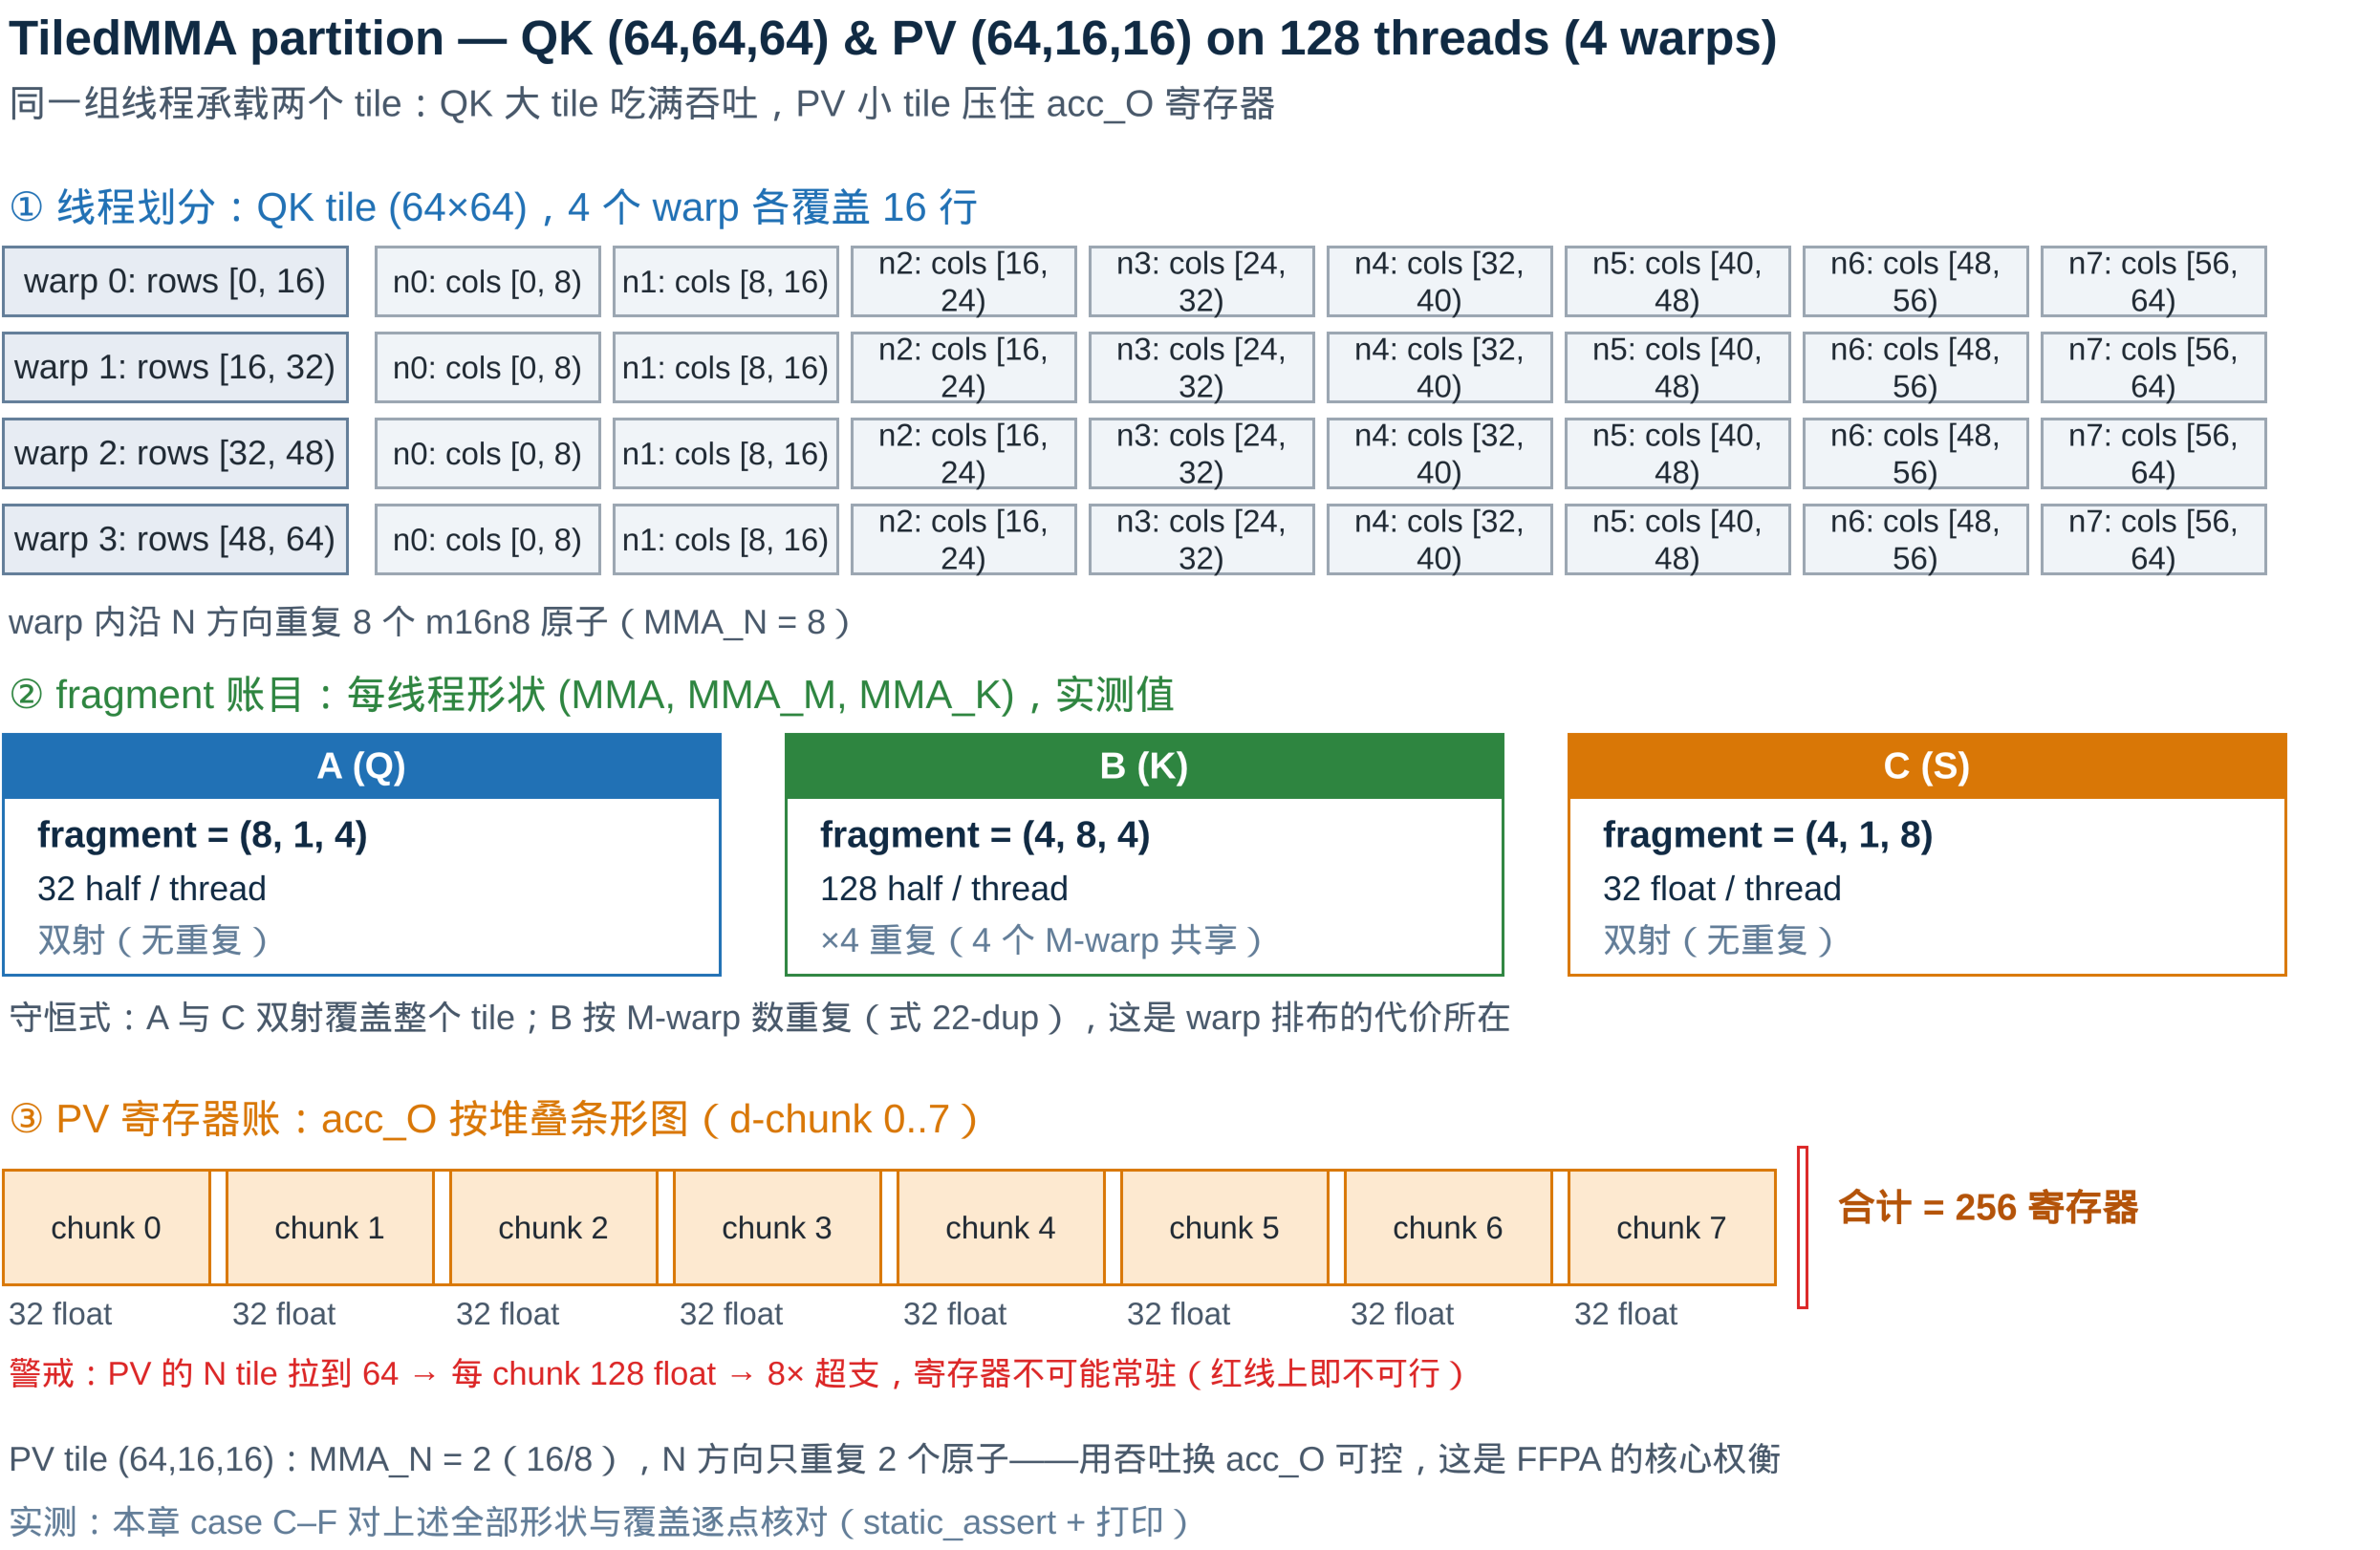
\includegraphics[width=0.92\textwidth]{figures/drawio/fig-22-1-tiledmma/fig-22-1.png}
\caption{TiledMMA partition：QK 的 $64\times64$ tile 上，4 个 warp 各覆盖
16 行，warp 内 N 方向重复 8 个原子；A/B/C 三种 fragment 的每线程形状与
重复因子（式~\eqref{eq:22-dup}）。下半部分是 PV 的 $(64,16,16)$ tile：
N 方向只重复 2 个原子，代价换来 per-call C 视图与拷贝粒度可控（8 个
d-chunk 各自拷回，常驻 acc\_O 256 寄存器不变；N tile 拉到 64 只是单次
调用的 C fragment 临时 4 倍）。本章测试 case~C--F
对全部形状与覆盖做了逐点核对。}
\label{fig:22-1}
\end{figure}

\begin{figure}[htbp]
\centering
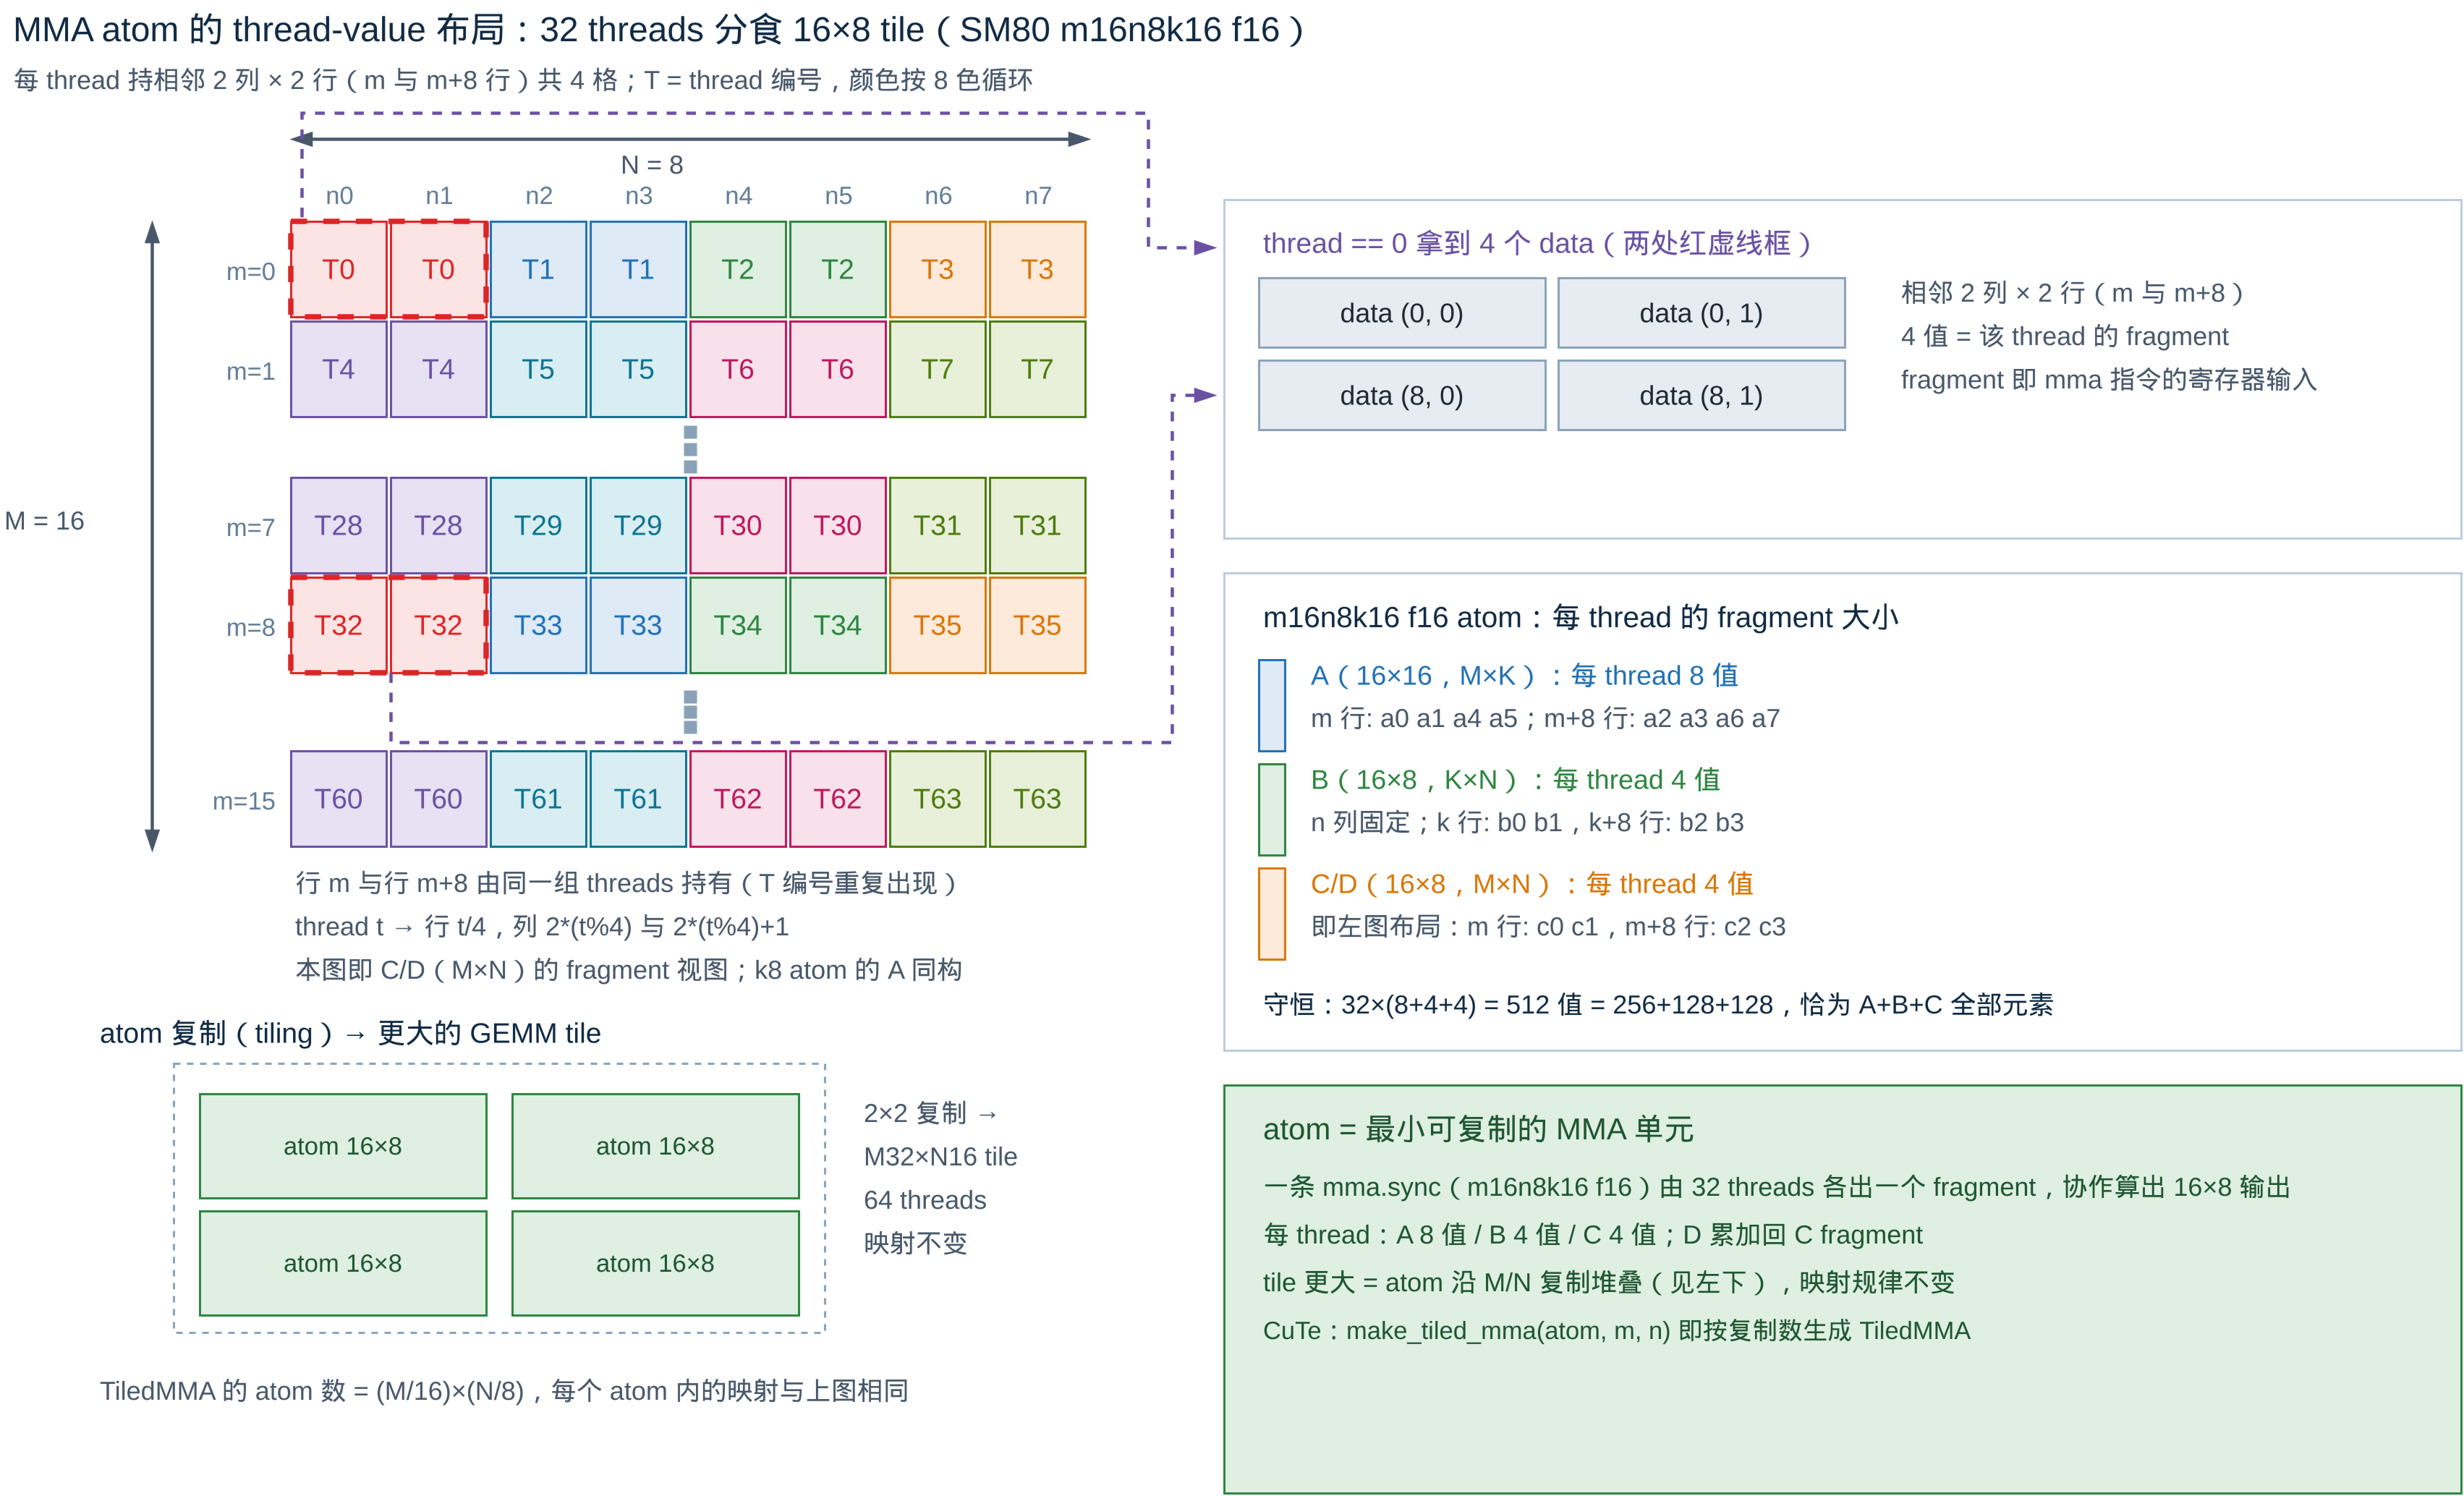
\includegraphics[width=0.95\textwidth]{figures/drawio/fig-22-2-mma-atom-fragments/fig-22-2.png}
\caption{m16n8k16 atom 的 C fragment thread-value 映射：thread $t$ 持行 $t/4$ 与 $t/4+8$、列 $2(t\bmod 4)$ 与 $2(t\bmod 4)+1$ 共 4 值——行 $m$ 与 $m+8$ 由同组线程重复持有。三个操作数每线程 A 8 值 / B 4 值 / C 4 值，守恒式 $32\times(8+4+4)=512$。更大的 tile 只是 atom 沿 M/N 的复制堆叠，thread-value 规律不变——\texttt{make\_\allowbreak{}tiled\_\allowbreak{}mma} 的构造基础。重建自 @竹熙佳处《写给大家看的 CuTe 教程：tiled mma》。}
\label{fig:22-2}
\end{figure}

\section{性能分析}

本章同样没有独立 bench：TiledMMA 的开销体现在它选择的 tile 形状上，端到端
数字在第~\ref{ch:19}、\ref{ch:26}~章（FFPA）与第~\ref{ch:24}~章（HGEMM）。
本节把「tile 选择」翻译成三条可计算的账。

\textbf{账一（寄存器）}：acc\_O $=kD_{\mathrm{chunks}}\times\mathrm{ThrLD}
\times\mathrm{MMA}_M\times\mathrm{MMA}_N\times\mathrm{Nrep}$（ThrLD 是单个
atom 每线程的 C 值数 $4$，Nrep 是 chunk 内 N 方向的重复数 $64/16=4$）
$=8\times4\times1\times2\times4=256$。PV 的
$\mathrm{MMA}_N = 2$（$16/8$）时每个 $64\times64$ d-chunk 每线程是 32 个
float；$D=512$ 时 $8$ 个 chunk 共 256 个寄存器。tile N=64 时单次 gemm 调用
的 C fragment 从 8 值涨到 32 值（4 倍），常驻 acc\_O（8 chunk $\times$ 32
$=$ 256 float）不变——超支的是每次调用的临时视图与 B fragment，不是
累加器。FFPA 注释「PV 保持小 tile」的算术依据正在于此：压的是每次调用的
临时开销，而非 acc\_O。

\textbf{账二（重复因子）}：B 的 fragment 按 M-warp 数重复（式~\eqref{eq:22-dup}）。
QK 用 $(4,1,1)$ 排布时 B 重复 4 倍（$4\times32=128$ 个 half/线程），
A 不重复；若改成 $(2,2,1)$（各方向 2 个 warp），A 与 B 各重复 2 倍——
总寄存器开销几乎不变，但 warp 覆盖的行会从 16 行变成 32 行。warp 排布的选择
因此是「谁重复」的问题，而不是「重复多少」的问题。

\textbf{账三（指令数）}：一次 TiledMMA 调用的指令数
$=\mathrm{MMA}_M\times\mathrm{MMA}_N\times\mathrm{MMA}_K$——注意这是
\emph{每线程（每 warp）}的条数。QK 的 $(1,8,4)=32$ 条是每个 warp 的量，
覆盖该 warp 的 $16\times64\times64$；4 个 warp 共 128 条才铺满 CTA 的
$64\times64\times64$——512 KFLOP/128 条，每条 $16\times8\times16$ 共
$4096$ FLOP（约 4.1 KFLOP）；PV 同口径：$(1,2,4)=8$ 条/warp 覆盖
$16\times16\times64$，CTA 的 $64\times16\times64$ 需 4 warp 共 32 条。
两个 tile 都让「每条 MMA 指令」吃满原子尺寸，没有浪费——因为它们都是从
$\mathrm{AtomShape}$ 出发、只用排布与 tile 尺寸做整数分块推出来的。

\textbf{口径说明}：本节所有数字都是 host 端类型推导的实测值（
\texttt{partition\_\allowbreak{}fragment\_\allowbreak{}*} 的形状），不含计时数据；FFPA 的
TFLOPS 对照见第~\ref{ch:19}~章的表与第~\ref{ch:26}~章的 kernel 分析。
还有一条引用纪律：ffpa\_attn.cuh L16--18 的头注释给出「SM120a
RTX PRO 5000：cuDNN SDPA 57.2 TFLOPS、FFPA TMA WS 110.7 TFLOPS（1.94x）」，
除法自洽（$110.7/57.2=1.94$），但设备口径是 \emph{RTX PRO 5000}（本机），
与 README 的 5090 口径不同——\textbf{引用这类比值时必须带上设备名}，
同一份代码在两块卡上的比值并不相等。

\section{常见坑}

\textbf{坑一：fragment 必须先清零/初始化。}
\texttt{partition\_\allowbreak{}fragment\_\allowbreak{}C} 返回的是「一块未定义的寄存器数组」的视图，
\emph{不会}置零。FFPA 里 \texttt{tCrS} 定义后立即 \texttt{clear(tCrS)}，
acc\_O 用显式循环清零（L173--176）。漏掉这一步的后果不是崩溃，而是把
未初始化寄存器当累加初值——编译器还可能把整个累加链折叠成垃圾值，
表现为「结果偶尔对、偶尔全错」。同理，被 \texttt{convert\_\allowbreak{}layout\_\allowbreak{}acc\_\allowbreak{}Aregs}
重解释的 $P$ 必须确保所有 32 个槽位都已被 softmax 写过。

\textbf{坑二：两个 TiledMMA 的 fragment 不能互换。}
QK 的 C fragment 是 $(4,1,8)$，PV 的 A fragment 是 $(8,1,4)$——形状、元素
类型（float/half）都不同。FFPA 的复用之所以成立，是因为它做了
\emph{类型转换 $+$ 布局重解释}两步（\texttt{convert\_\allowbreak{}type} $+$
\texttt{convert\_\allowbreak{}layout\_\allowbreak{}acc\_\allowbreak{}Aregs}），且只对 m16n8k16 这一族成立。
把 C 直接喂给 PV 是经典的静默错位。

\textbf{坑三：tile 必须是原子的整数倍，warp 排布必须与线程数自洽。}
$\mathrm{perm\_M}$ 不是 $16$ 的倍数、或 $\mathrm{ThrM}\times 32$ 与
\texttt{blockDim} 不一致时，partition 会产生多余/缺失的 remainder mode
（编译期静态断言或运行期越界）。判据：\texttt{size(mma)} 是线程数的权威，
用它来配 \texttt{dim3 block\allowbreak{}(size\allowbreak{}(mma))}。

\textbf{坑四：\texttt{get\_slice} 的坐标是 $(\mathrm{ThrV},(\mathrm{ThrM},
\mathrm{ThrN/K}))$ 三层，不是「warp 内 lane $+$ 全局 warp」两层。}
FFPA 的 $128$ 线程排布是 $(\mathrm{ThrV}=32,\mathrm{ThrM}=4)$，因此
线程 $t$ 的行带是 $16\lfloor t/32\rfloor$——把 $\mathrm{ThrM}$ 当成
「线程号对 4 取模」会得到完全错误的 warp 映射（本章测试 case~E 专门核对
这条）。

\textbf{坑五：\texttt{partition\_\allowbreak{}fragment\_\allowbreak{}A} 的输入决定 fragment 的
MMAK 大小，但不改变 atom 约定。}
QK 的 A 在 $(64,64)$ 上是 $(8,1,4)$，在 $(64,16)$ 上就是 $(8,1,1)$；
$\mathrm{MMA}_K$ 随输入 K 长度变化。写循环时要用
\texttt{size\allowbreak{}<2>\allowbreak{}(fragment)} 作为 K 循环上界（第~\ref{ch:21}~章 kernel 的
\texttt{num\_k\_steps} 就是这么来的），不要写死。

\textbf{坑六：C fragment 的「行列」不是直觉顺序。}
$(4,1,8)$ 的 4 个 float 对应「2 行 $\times$ 2 列」，同一个 lane 的第 0、1 个
元素在同一行相邻两列，第 2、3 个在 $+8$ 行处。想按 (row, col) 遍历必须先做
\texttt{convert\_\allowbreak{}layout\_\allowbreak{}acc\_\allowbreak{}rowcol}（L2315--2333 推导）；直接用
\texttt{fragment\allowbreak{}(idx)} 当矩阵元素是最常见的读错方式。

\section{面试要点速查}

\textbf{Q1：MMA\_Atom 与 TiledMMA 的区别？}\\
A：MMA\_Atom 是一条指令的抽象（Shape\_MNK $+$ 三份 TV layout $+$ ThrID）；
TiledMMA 是「把原子铺满一个 tile」的类型，多出 warp 排布与 tile 尺寸两个
参数，并提供 \texttt{partition\_\allowbreak{}fragment\_\allowbreak{}*}。

\textbf{Q2：\texttt{make\_\allowbreak{}tiled\_\allowbreak{}mma} 的第二个、第三个参数分别是什么？}\\
A：第二个是 warp 排布（\texttt{Atom\allowbreak{}Layout\allowbreak{}MNK}，决定 \texttt{Thr\allowbreak{}M/\allowbreak{}Thr\allowbreak{}N/\allowbreak{}Thr\allowbreak{}K}
与重复因子），第三个是目标 tile 尺寸（\texttt{Permutation\allowbreak{}MNK}，含 K）。
FFPA：排布 $(4,1,1)$，tile $(64,64,16)$ 与 $(64,16,16)$。

\textbf{Q3：fragment 的三个 mode 是什么？}\\
A：$(\mathrm{MMA}, \mathrm{MMA}_M, \mathrm{MMA}_K)$——每个原子的值数、
M 方向原子重复、K 方向原子重复（C 的第三 mode 是
$\mathrm{MMA}_N$）。它们是式~\eqref{eq:22-thrfrg-4} 第 (4) 步之后的余量。

\textbf{Q4：为什么 A 的 fragment 有时会重复？}\\
A：warp 排布如果在 N 方向有分片，不同 N-warp 需要同一份 A，于是 A 被
重复持有（重复因子 $=$ N-warp 数）；B 同理（因子 $=$ M-warp 数）。
式~\eqref{eq:22-dup}。

\textbf{Q5：\texttt{get\_\allowbreak{}slice\allowbreak{}(t)} 内部发生了什么？}\\
A：把整数 $t$ 按 \texttt{Thr\allowbreak{}Layout\allowbreak{}VMNK} 分解成
$(\mathrm{ThrV},(\mathrm{ThrM},\mathrm{ThrN}),\mathrm{ThrK})$，得到一个
「只属于该线程」的 ThrMMA，后续 partition 都基于它。

\textbf{Q6：QK 与 PV 为什么要用两个 TiledMMA？}\\
A：目标不同。QK 要一次覆盖整个 $S$（N $=64$）省循环；PV 的 N 直接决定
acc\_O 的寄存器数，必须小。两者共享同一套 128 线程排布，fragment 通过
类型转换 $+$ 布局重解释衔接。

\textbf{Q7：\texttt{tile\_\allowbreak{}size\allowbreak{}<I>\allowbreak{}(mma)} 有什么用？}\\
A：它是 TiledMMA 对外的尺寸接口，也是 \texttt{make\_\allowbreak{}tiled\_\allowbreak{}copy\_\allowbreak{}A/\allowbreak{}B/\allowbreak{}C}
推导 S$\to$R 拷贝 tiler 的来源（第~\ref{ch:21}~章式~(21-mtca)）——
TiledMMA 与 TiledCopy 通过它解耦：改 tile 不影响拷贝代码。

\textbf{Q8：tile 的 N 尺寸调节什么？}\\
A：单次调用 C fragment 每线程元素数 $=\mathrm{MMA}\times\mathrm{MMA}_M\times
\mathrm{MMA}_N$，而 $\mathrm{MMA}_N = \mathrm{tile}_N/\mathrm{atom}_N$——
tile N 增大时 per-call C 视图与 B fragment 随之线性增长，S$\to$R 拷贝
粒度变粗；常驻 acc\_O（$D=512$ 时 256 个寄存器）不变，PV 因此取
$\mathrm{tile}_N=16$（$64\times16\times16$）。

\section{最小测试与动手实验}

测试文件：\texttt{book/\allowbreak{}tests/\allowbreak{}ch22\_\allowbreak{}tiled\_\allowbreak{}mma.cu}（host-only：只做类型与
partition 断言，不启动 kernel；直接 include
\texttt{.\allowbreak{}.\allowbreak{}/\allowbreak{}.\allowbreak{}.\allowbreak{}/\allowbreak{}ffpa\_\allowbreak{}attn.\allowbreak{}cuh} 以核对真实的 traits）。六个 case：

\begin{itemize}
  \item \textbf{A 原子 fragment 公式}：对
        \texttt{SM80\_\allowbreak{}16x8x16\_\allowbreak{}F32\allowbreak{}F16\allowbreak{}F16\allowbreak{}F32\_\allowbreak{}TN} 的 A/B/C 三个 layout，
        逐 lane、逐值核对手推公式式~\eqref{eq:22-atom-a}--\eqref{eq:22-atom-c}
        （$32\times8$、$32\times4$、$32\times4$ 个断言）；
  \item \textbf{B tile\_size 与线程数}：QK/PV 的 \texttt{tile\_size} 为
        $(64,64,16)/(64,16,16)$、\texttt{size(mma)}$=128$；对象
        \texttt{FFPAAttn\allowbreak{}Split\allowbreak{}DCu\allowbreak{}Te\allowbreak{}Traits\allowbreak{}<512>}
        并与手写的
        \texttt{make\_\allowbreak{}tiled\_\allowbreak{}mma} 构造做类型一致性检查；
  \item \textbf{C fragment 形状}：QK 在 $(64,64)$ 上 A/B/C 每线程
        $(8,1,4)/(4,8,4)/(4,1,8)$，PV 为 $(8,1,4)/(4,2,1)/(4,1,8)$；
        逐项核对元素数；
  \item \textbf{D 守恒与重复因子}：C 的覆盖是双射（$128\times32=4096=
        64\times64$）且 A 也是；B 恰好 4 倍重复（每元素被 4 个
        (线程, 值) 对覆盖）；
  \item \textbf{E warp 边界}：QK 的 C fragment 逐线程回投坐标，四个 warp 的
        行带为 $[0,16),[16,32),[32,48),[48,64)$，互不重叠；
  \item \textbf{F PV 的 acc\_O 账目}：
        \texttt{partition\_\allowbreak{}fragment\_\allowbreak{}C\allowbreak{}(tiled\_\allowbreak{}mma\_\allowbreak{}pv,\allowbreak{} Shape\allowbreak{}<\_\allowbreak{},\allowbreak{}64,\allowbreak{}\_\allowbreak{}64>\{\})}
        每线程 32 个值，$\times$ 8 个 d-chunk（$D=512$）$=256$ 个寄存器——
        与源码注释的寄存器压力说法互证；并核对 PV 的 C 覆盖
        （$64\times16$ 双射）。
\end{itemize}

运行命令：

\begin{lstlisting}[style=console]
cd kernels/interview/book/tests
CUDA_VISIBLE_DEVICES=6 ./build_tests.sh --arch sm_120a --ch ch22
\end{lstlisting}

预期输出（本机 RTX PRO 5000，CUDA 13.2，CUTLASS v4.6.1，2026-09-11 实测）：

\begin{lstlisting}[style=console]
ch22 CuTe TiledMMA & fragments (host-only, no kernel launch)
PASS case A MMA atom fragment layouts (m16n8k16): mismatches=0 (519 checks)
PASS case B FFPA traits tile_size & thread count: mismatches=0 (14 checks)
PASS case C partition_fragment shapes QK/PV: mismatches=0 (12 checks)
PASS case D conservation & B duplication factor: mismatches=0 (4 checks)
PASS case E warp row bands & cross-warp boundary: mismatches=0 (4360 checks)
PASS case F PV acc_O register budget & coverage: mismatches=0 (136 checks)
ALL OK
\end{lstlisting}

动手实验：

\begin{enumerate}
  \item 把 case~C 的 PV mma 的 tile 从 \texttt{Tile\allowbreak{}<64,\allowbreak{}16,\allowbreak{}16>} 改成
        \texttt{Tile\allowbreak{}<64,\allowbreak{}32,\allowbreak{}16>}，观察 fragment 的 $\mathrm{MMA}_N$ 从 2 变
        4、单次调用的 C 视图从 8 涨到 16 个值，而单个 d-chunk 的 acc\_O
        仍是 32——亲手体验「tile N 调节 per-call C 视图与拷贝粒度」；
  \item 把 QK 的 warp 排布从 \texttt{Layout\allowbreak{}<Shape\allowbreak{}<\_\allowbreak{},\allowbreak{}4,\allowbreak{}\_\allowbreak{},\allowbreak{}\_\allowbreak{}>>} 改成
        \texttt{Layout\allowbreak{}<Shape\allowbreak{}<\_\allowbreak{},\allowbreak{}2,\allowbreak{}\_\allowbreak{}2,\allowbreak{}\_\allowbreak{}>>}（$2\times2$ 网格），观察
        A/B 的重复因子与 warp 行带如何变化（case~D/E 的断言会同时失效，
        这正是要看的现象）；
  \item 把 case~A 的 lane 换成 $32+k$ 或把值编号顺序反转，确认断言能立刻
        抓到错误——用来理解「formula-driven 测试」与「只比形状」的差别。
\end{enumerate}

\section*{延伸阅读}

\begin{itemize}
  \item @竹熙佳处《写给大家看的 CuTe 教程：Tiled MMA》，
        \url{https://zhuanlan.zhihu.com/p/1937145378446226159}
        （本计划的 ch22 主参考；素材清单标注「待核」，本章全部结论以
        CUTLASS v4.6.1 头文件实测为准）；
  \item @reed《cute 之 MMA 抽象》，
        \url{https://zhuanlan.zhihu.com/p/663092747}
        （MMA\_Atom/MMA\_Traits 的设计动机与历史，读 3.1--3.2 节时对照）；
  \item @可怕的杰瑞《Cute TiledMMA 简单理解》，
        \url{https://zhuanlan.zhihu.com/p/1991908850132088026}
        （用可编译的最小例子演示 make\_tiled\_mma 的三个参数，
        与本章 case~B 的实验同构；续篇
        \url{https://zhuanlan.zhihu.com/p/1992328297888126320}）；
  \item @水木皇工仔《基于 CuTe 理解 swizzle, LDSM, MMA》，
        \url{https://zhuanlan.zhihu.com/p/934430036}
        （把 LDSM 的 lane 映射与 MMA fragment 放在一起推，与第~\ref{ch:21}~章
        case~D、本章 case~A 互补）。
\end{itemize}

